\chapter{Fundamentos teóricos eléctricos.}
\section{Campo eléctrico y campo magnético.}\label{sec:Campo electrico y campo magnetico.}
\setcounter{equation}{0}
\setcounter{figure}{0}
Es importante tener claros los conceptos de campo eléctrico y campo magnético antes de adentrarnos en el problema. En esta sección veremos la definición de ambos campos, sus propiedades y un esquema ilustrativo, para ayudar a entender de mejor manera estas ideas.
\subsection{Campo eléctrico.}
Como definición el campo eléctrico es 'Campo físico que describe la interaccón entre 2 cuerpos o sistemas con propiedades de naturaleza eléctrica'. Está representado por la letra $E$, también se podría definir como la fuerza eléctrica $F_{e}$  por unidad de carga $q$ o bien:
$$E=\frac{F}{q}$$
El campo eléctrico estático puede representarse esquemáticamente a tráves de líneas, conocidas como \textbf{líneas de campo}.
\begin{figure}[H]
\centering
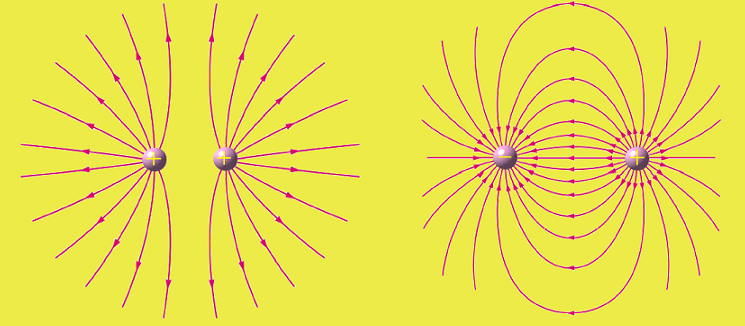
\includegraphics[height=8cm]{Imagenes/Lineas_de_campo.png}
\caption{Líneas de campo eléctrico. (Fuente: \cite{serway2015fisica})}\label{fig:Lineas de campo electrico}
\end{figure}
Las líneas de campo eléctrico poseen las siguientes carácteristicas:
\begin{itemize}
\item El vector de campo eléctrico en cualquier punto es tangente a la línea que pasa por dicho punto.
\item Las líneas de campo no se cruzan.
\item El número de líneas que salen de una carga positiva o entran en una carga negativa es proporcional a dicha carga.
\item Las líneas de campo no pueden cortarse. De lo contrario en el punto de corte existirían dos vectores campo eléctrico distintos.
\item A grandes distancias de un sistema de cargas, las líneas están igualmente espaciadas y son radiales, comportándose el sistema como una carga puntual.
\end{itemize}
\subsection{Campo magnético.}
El campo mágnetico, al igual que el campo eléctrico es una magnitud vectorial. Es generado por cargas en movimiento, estas pueden ser puntuales o un conjunto de cargas o en otras palabras, una corriente eléctrica. Su unidad de medida es el tesla $(T)$.\\
El movimiento de una carga puntual produce un campo magnético de la forma:
\begin{figure}[H]
\centering
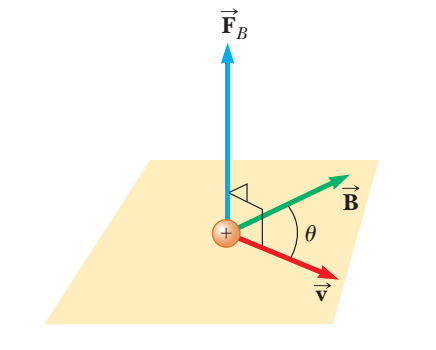
\includegraphics[height=6cm]{Imagenes/campomag.png}\caption{Campo magnético por una carga puntual. (Fuente: \cite{serway2015fisica})}\label{fig:Campo magnetico}
\end{figure}
El campo magnético viene dado por:
$$\overrightarrow{B}=\frac{\mu_0}{4\pi}\,\frac{q\,\overrightarrow{v}\times\overrightarrow{u_r}}{r^2}$$
Donde $q$ es la carga puntual que crea el campo, $v$ es la velocidad de $q$, $r$ es la distancia desde $q$ hasta $P$, $P$ es el punto donde estamos calculando el campo magnético, $u_r$ es un vector unitario que va desde $q$ hasta $P$, $μ_0$ es una constante denominada permeabilidad del espacio libre. Su valor en el Sistema Internacional es $μ_0 = 4 \pi 10^{-7} T m/A$.\\
Por otro lado, una corriente eléctrica son muchas cargas puntuales moviendose en conjunto, por lo que también generan un campo magnético. En este caso el calculo del campo será con elementos infinitesimales:
\begin{figure}[H]
\centering
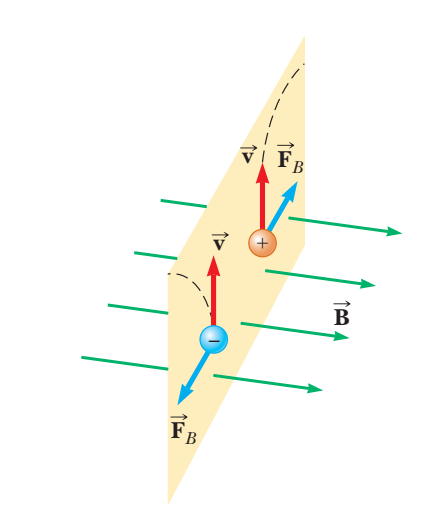
\includegraphics[height=8cm]{Imagenes/campomag_corr.png}\caption{Campo magnético por una corriente eléctrica. (Fuente: \cite{serway2015fisica})}\label{fig:Campo magnetico por una corriente}
\end{figure}
En donde $I$ es la intensidad de la corriente, dada por la fórmula $I=q\,n\,v_d\,A$, con $n$ siendo la cantidad de cargas, $A$ la sección del hilo y $v_d$ la velocidad del desplazamiento.
$$d\overrightarrow{B}=\frac{μ_0}{4\pi}\, \frac{I\,\overrightarrow{dl}\times \overrightarrow{u_r}}{r^2} $$
\subsection{Leyes de Maxwell.}\label{sec:Leyes de Maxwell}
Como vimos anteriormente existen campos eléctricos y campos magnéticos, el conjunto de ambos campos se conoce como campo electromagnético. A tráves de este campo, los elementos que interactúan entre si por medio de la electricidad o el magnetismo se comportan siguiendo ciertas reglas de como los elementos perturban al campo, o como el campo se perturba a si mismo. Estas reglas son conocidas como las ecuaciones o leyes de Maxwell.\\
En un principio eran 8, luego se condensaron en 4 y se pueden escribir como: 
\begin{equation}
\label{eq:maxwell1}
\vec {\nabla} \cdot\vec{E}=\frac{\rho}{\varepsilon_0}\\
\end{equation}
\begin{equation}
\label{eq:maxwell2}
\vec {\nabla} \cdot\vec{B}=0\\
\end{equation}
\begin{equation}
\label{eq:maxwell3}
\vec {\nabla} \times\vec{E}=-\frac{\partial \vec{B}}{\partial t}\\
\end{equation}
\begin{equation}
\label{eq:maxwell4}
\vec {\nabla} \times\vec{B}=\mu_0\vec{J}+\mu_0\varepsilon_0\frac{\partial \vec{E}}{\partial t}\\
\end{equation}
Para entender un poco más las ecuaciones, pasaremos a explicaralas. La ecuación \eqref{eq:maxwell1} también conocida como la \textbf{Ley de Gauss} nos dice básicamente que las cargas positivas serán fuentes y que las cargas negativas serán sumideros, tal cual como se ve en la imagen \ref{fig:Lineas de campo electrico}, en otras palabras, cargas del mismo signo repelen y cargas opuestas se atraen, notar que $\rho$ es la densidad de carga y $\varepsilon_0$ es la permitividad eléctrica en el vacío. Esta ley también nos indica que el campo eléctrico decae con la distancia, lo hace a razón de $1/r^2$. La ecuación \eqref{eq:maxwell2}, algo así como la Ley de Gauss del magnetismo, indica que no hay fuentes o sumideros de campo magnético, lo que no impide que hayan elementos que generen campos magneticos, como vimos anteriormente. ¿Por qué es importante esto? Porque nos indica que el campo magnético siempre debe cerrarse sobre si mismo. De forma práctica esto se ve al cortar un imán por la mitad, si bien en un inicio solo existe un polo sur y otro norte, al cortarlo en 2 cada trozo tiene su polo sur y norte respectivamente. Es decir, los monopolos no existen. La ecuación \eqref{eq:maxwell3}, también conocida como la \textbf{Ley de Faraday}  nos dice que si un campo magético cambia en el tiempo este 'activa' el campo eléctrico, por lo tanto no solo las cargas e imanes influyen en los campos sino que estos influyen entre si, lo que nos lleva directamente a la ecuación \eqref{eq:maxwell4} o la \textbf{Ley de Ampère-Maxwell} que también nos dice que si el campo eléctrico cambia en el tiempo o cargas moviendose, es decir una corriente eléctrica denotada en la ecuación como $\vec{J}$, esto activará el campo magnético. Las constantes utilizadas en las ecuaciones son:
\begin{itemize}
\item Permitividad eléctrica en el vacío
$$\varepsilon_0=8.85\times 10^{-12} \left[\frac{C^2}{N\cdot m^2}\right]$$
\item Permisividad magnética en el vacío
$$\mu_0=4 \pi \times 10^{-7}\left[\frac{N}{A^2}\right]$$
\end{itemize}

Combinando estas 4 leyes es válido decir que todos los fenómenos electromagnéticos que percibimos se pueden explicar. 
\begin{figure}[H]
\centering
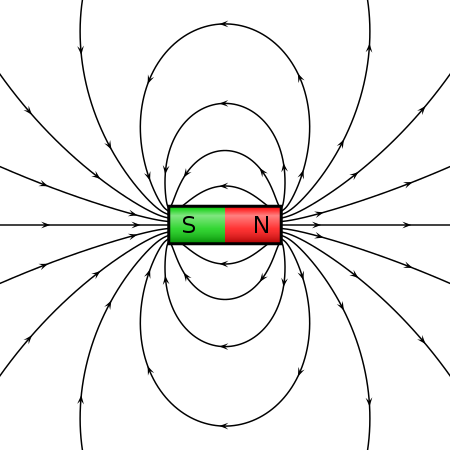
\includegraphics[height=7cm]{Imagenes/lineasmag.png}\label{fig:Lineas de campo magnetico}
\caption{Líneas de campo magnético. (Fuente: \cite{serway2015fisica})}
\end{figure}
Las ecuaciones descritas con anterioridad son dadas para el medio vacío. Para el caso en que los elementos se encuentre en un medio es necesario adaptar las propiedades del mismo. Se pueden encontrar una nueva relación para $E$ y $B$ a través de dos parámetros ya conocidos, como permitividad eléctrica y permisividad magnética. La relación es de la forma:
$$\vec{E}=\frac{\vec{D}}{\varepsilon}$$
$$\vec{B}=\mu \vec{H}$$
En donde $D$ se define como la densidad el flujo eléctrico y $H$ como la intensidad del campo magnético. Se dice que si la relación entre  $E/D$ y $B/H$ estamos en presencia de un medio lineal. Esto permite que $\varepsilon$ y $\mu$ se representen de forma matricial. Si esta matriz se puede diagonalizar, es decir que que solo existan en la diagonal se habla de un medio isótropo y si además los elementos no son iguales se habla de un medio anisótropo. Un elemento isótropo es un elemento en el que sus cualidades físicas no dependen de la dirección en la que son examinadas, por el contrario en el anisótropo su dirección varía sus propiedades físicas.

\begin{figure}[H]
\centering
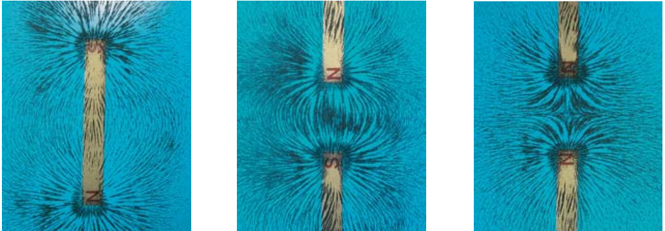
\includegraphics[height=5.5cm]{Imagenes/camposmag.png}\label{fig:Ejemplos de campos magneticos}
\caption{Líneas de campo magnético. (Fuente: \cite{serway2015fisica})}
\end{figure}
Es necesario notar que una onda electromagnética puede propagar a su vez un campo electromagnético, el cúal se puede descomponer de un campo eléctrico y uno magnético, los cuales son perpendiculares entre si y entre la dirección de propagación. Tal como se muestra en la figura siguiente:
\begin{figure}[H]
\centering
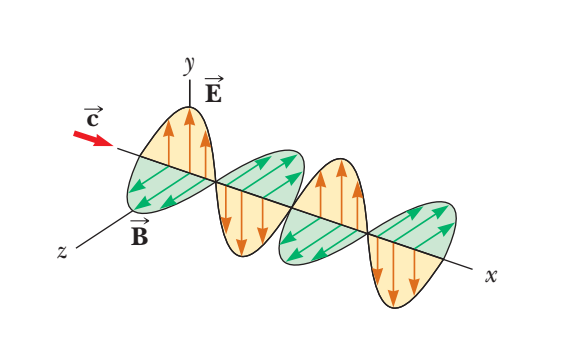
\includegraphics[height=7cm]{Imagenes/ondaelectromagneticas.png}\label{fig:Onda electromagnetica}
\caption{Propagación de onda electromagnética. (Fuente: \cite{serway2015fisica})}
\end{figure}
